\begin{abstract}
Neural network applications of ever-growing size and their adaptations for a growing number of different and sometimes less powerful devices necessitate pruning; The reduction in network size through the removal of superfluous substructures. The term pruning usually implies that the network in question has absolved training until convergence; techniques for a-priori reductions are generally referred to as network architecture search.\\
While most pruning techniques retain the weights of the trained network, in their paper "The Lottery Ticket Hypothesis: Finding Sparse, Trainable Neural Networks," J. Frankle and M. Carbin present a novel technique which resets the weights of the pruned network to their pre-training values.\\
\\
The primary aim of this thesis is to extend their work and research whether the presented algorithm can provide competitive pruning on different datasets, specifically in the field of natural language processing. As the reset to initial values leaves said algorithm similar to a network architecture search method, the pruning can be interpreted as a search dependant on the weights of the trained network. This work also studies how this search develops in quality over the amount of training provided beforehand.\\
\\
In pursuit of these two goals, we developed a framework through in we implemented four experiments. The first two experiments aimed to confirm the validity of the codebase. Subsequently, the third one intended to establish an argument for application of their pruning method in the field of natural language processing. With the last experiment, we plan to provide explorative data to inform further study on the emergence of actionable experience in the values of a network.\\
\\
While the first two experiments failed to reproduce the results of J. Frankle and M. Carbin, one of them pruned its associated network up to the scale of contemporary technique. It achieved a size reduction of 90 percent with little loss in accuracy. Additionally, the third result conforms with their definition of a lottery ticket, producing the same or even better quality measure, up to the same degree of compression. Finally, the data of the exploratory experiment show low legibility due to the erratic results of single prunings. Nonetheless, none of the early pruning trials achieve the same level of accuracy displayed by our previous experiment, even if the latter trials pruned as late as epoch 10, an amount of training for which the full network already converged. These results suggest that, during the pruning iterations,  the pruning algorithm has to submit a given network to more training than necessary for primary convergence. 
\end{abstract}




%*****************************************
%*************Introduction****************
%*****************************************
%*****************************************
\chapter{Introduction}
%*****************************************
The thesis on hand discusses the possible extensions of a specific neural network pruning technique presented by J. Frankle and Michael at the beginning of 2019. [cite LTH]\\
The next few paragraphs motivate the research,  specify its extent, and give an outline for the remaining chapters.

\section{Motivation}
Over the last decade, neural networks have become ever more prevalent in applications of any kind. Not only can they theoretically approximate most mappings between inputs and expected output[footnote] up to arbitrary precision[footnote], but in practice, they can also converge on such an approximation via gradient descent.\cite{?}\\ 
As computational resources became more available, state-of-the-art approaches featured ever-larger networks. Although they excel at their tasks, it is challenging to execute them on small portable devices such as smartphones. Pruning techniques aim to reduce the size architectures have at runtime through the removal of parts that are no longer necessary after training. Still, there is no consesus on how to identify these superfluous sections.\\
In their paper "The Lottery Ticket Hypothesis: Finding Sparse, Trainable Neural Networks," J. Frankle and M. Carbin demonstrate an innovative algorithm to remove up to 90 percent of various networks while retaining most or all of their performance. These results are comparable to other pruning techniques while promising new insights into the nature of neural networks.\cite{LTH}
\\
The following chapters of this work explore the transfer of the Lottery Ticket Hypothesis to another field as well as earlier retrieval of lottery tickets on a previously studied architecture.

\section{Problem Statement and Contribution}
In the latter half of their paper, J. Frankle and M. Carbin discuss the limitations of their work. First and Foremost, they applied their method only to small datasets because iterative pruning is computationally expensive.\cite{LTH} Additionally, both datasets they studied are from the field of image recognition, and it is uncertain whether their results are transferable to other contexts such as natural language processing or voice recognition.\\
Furthermore, J. Frankle and M. Carbin acknowledge that pruning single connections instead of whole sections of a network does not line up well with modern frameworks, and thus, no actual speed-up is achieved. Finally, they state that they plan to research ways to find lottery tickets earlier or at smaller sizes.\cite{LTH}


\section{Outline}

After this introduction, chapter \ref{ch:background} of this thesis establishes the necessary background for the upcoming descriptions and discussions. Afterward, section \ref{ch:relatedwork} gives an overview of the work already done on the Lottery Ticket Hypothesis and the tasks absolved during the experiments. Chapter \ref{ch:design} describes the design of the experiments without mention of the implementation details, which follow in section \ref{ch:implementation}. Before the discussion of the results, chapter \ref{ch:datasets} supplies additional information on the datasets utilized in this thesis.\\
Finally, section \ref{ch:evaluation} presents an evaluation, and chapter \ref{ch:closure} conludes this work with a summary and a mention of possibilities for future work.

%*****************************************
%**************Background*****************
%*****************************************
%*****************************************
\chapter{Background}
\label{ch:background}
%*****************************************
\hint{This chapter should give a comprehensive overview on the background necessary to understand the thesis.
The chapter should have a length of about five pages!}


\section{Basics of Neural Networks\ \ \  \(WIP\)}
Neural networks are a part of most major AI-breakthrough in the last decade enabling computers to compete in fields formerly championed by humans.\footnote{
	\begin{itemize}
		\item 
			2011: "Watson" of IBM defeats two former grand champions in "Jeopardy!" \cite{lally2011natural}
		\item 
			2011: "Siri" enables users to use natural language to interact with their phones 
			\cite{ARON201124}
		\item 
			2015: A convolutional neural network classifies images from the ImageNet dataset more accurately than human experts 
			\cite{Russakovsky2015} \cite{He_2015_ICCV}
		\item 
			2016: "AlphaGo" beats Lee Sedol, one of the world's strongest Go players
			\cite{gibney2016google} \cite{silver2017mastering}
	\end{itemize}
}
They implement a statistical understanding of AI, which is to say that they try to find a specific model optimizing the likelihood of reproducing input-output pairs similar to some training data. The competing philosophy directly divines behaviour rules, frequently from expert knowledge, and as such is far less dependant from data.  
\textcolor{red}{[citation needed]}\\
For the former concept its model classes are the essential point of design. A multitude of properties maybe sought after in a model class of which a few important ones are:
\begin{itemize}
	\item \textbf{Richness:}\\
	The diversity of single models in the class and thus the ability to fit a wide field of different input-output landscapes.\footnote{
		More formally the richness of a model class can be described as the amount of different functions from the input-space to the output-space which can be expressed through a model of said class.}\\
	If a model class is inherently restricted the underlying relation between inputs and outputs might simply be beyond the expressive capabilities of all its models.\\
	In other words: If a model class is not rich enough all of its models will underfit the given training data.
	\item \textbf{Stability:}\\ 
	Tendency of similar models in the class to handle inputs in a similar way.\\
	If your model class shows unstable behavior defining a sensible way to search it for good models becomes difficult.
	\item \textbf{Interpretability of Models:}\\
	 Ease of formulating knowledge out of any given model in the class.\\
	 As fields exist in which statistical AI outperform experts the extraction of knowledge understandable and applicable by humans is of special interest.
	\item \textcolor{red}
	{[citation needed]}
\end{itemize}
If one knows an entity that already performs well on a given task it is a sensible approach to design ones model class to reproduce its decision process. Humans usually are such entities for many tasks of interest to AI research so they are a natural source of inspiration. Neural networks essentially are simplified models of a human central nervous system. \\
The most basic building block of the human central nervous system is a neuron which can receive multiple stimuli and is able to produce an output if the combined stimulation exceeds a threshold.\textcolor{red}{[citation needed]} One such neuron and its stimulus measure are depicted in \ref{fig:neuron1}. Another functionality observed in nature is the ability of a neuron to strengthen the connection to any source of stimulus thus giving said source more influence on whether the neuron produces an output. 
\textcolor{red}{[citation needed]}\\
\\
The canonical mathematical model of a neuron, as seen in \ref{fig:neuron2}, is defined as:
\begin{itemize}
	\item \textbf{Inputs} $x_i$ \textbf{:}\\
	All stimuli of a neuron are simply referred to as its inputs
	\item \textbf{Weights} $w_i$ \textbf{:}\\
	The ability to assign importances is modelled as weights which are coupled to specific stimuli
	\item \textbf{Combined Weighted Inputs} $\sum_{i=1}^{n}w_i x_i$ \textbf{:}\\
	After the inputs are scaled by their according weight they superpose to form the total excitation of the neuron
	\item \textbf{Activation Function} $\Phi(\sum_{i=1}^{n}w_i x_i)$ \textbf{:}\\
	...
	\item \textbf{Bias} $b$ \textbf{:}\\  
	...
\end{itemize}


\begin{figure}
	\centering
	\begin{minipage}{0.45\textwidth}
		\centering
		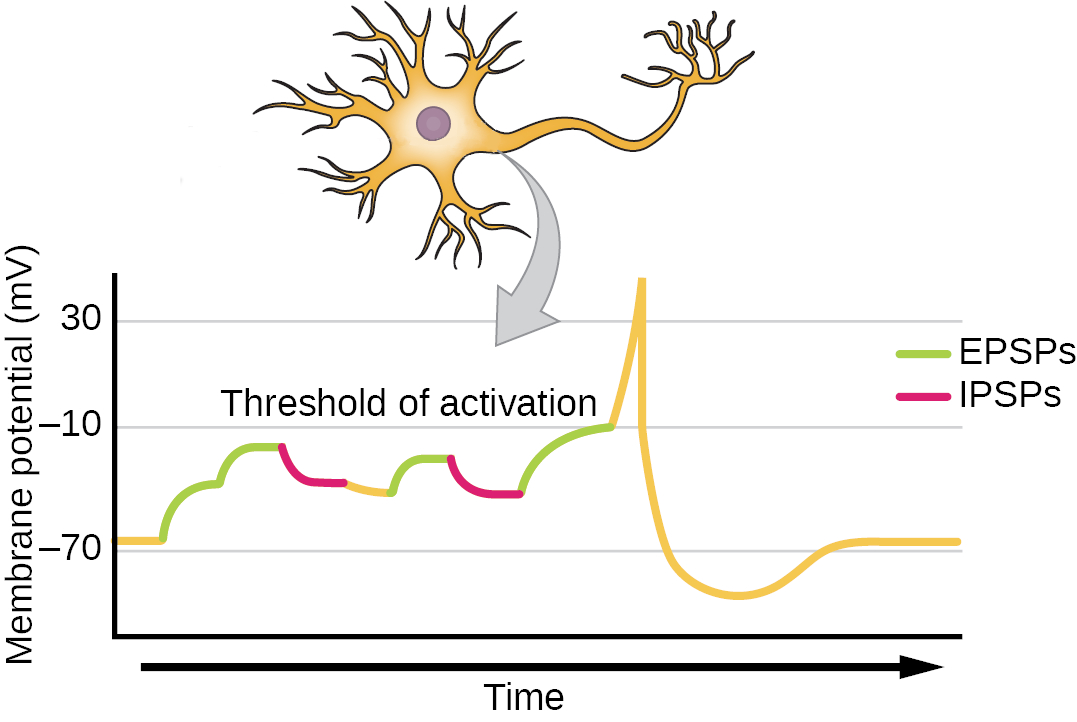
\includegraphics[height=150px]{gfx/Biological_Neuron_edited.jpg}
		\caption{Representation of a biological Neuron\\
			\cite{biology} edited}
		\label{fig:neuron1}
	\end{minipage}\hfill
	\begin{minipage}{0.45\textwidth}
		\centering
		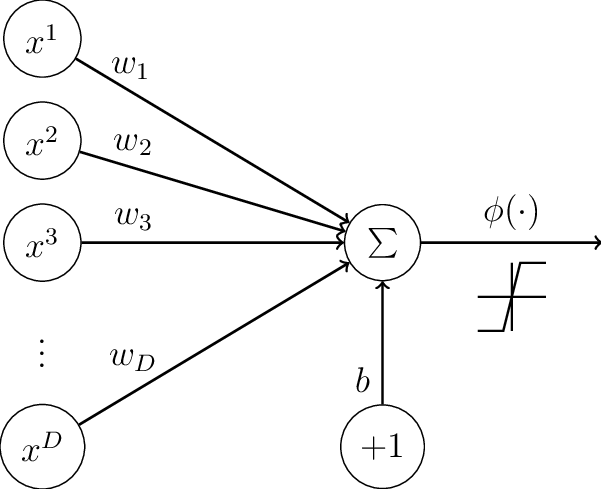
\includegraphics[height=150px]{gfx/Abstract_Neuron.png}
		\caption{Abstraction of a Neuron\\
			\cite{abstract_neuron}}
		\label{fig:neuron2}
	\end{minipage}
\end{figure}

As an individual neurons is too simple to model any complex relations between inputs
and outputs the next step is to aggregate multiple neurons. Figure \ref{fig:FFNetwork} displays a few neurons coming together to form a simple fully-connected feed-forward network.
\footnote{
	Inputs of neural networks are often called "features" and fully-connected networks are frequently referred to as "dense"	}
\begin{figure}
	\centering
		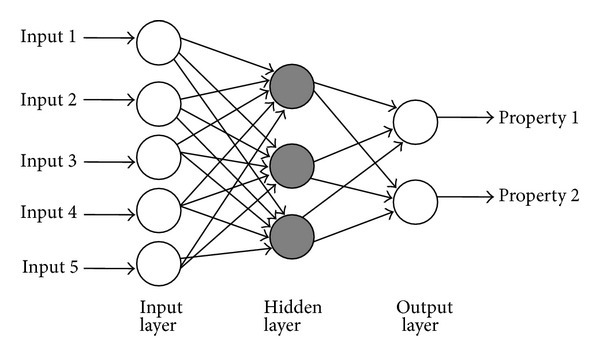
\includegraphics[height=150px]{gfx/Dense_FFNetwork.jpg}
		\caption{A small fully-connected network\\
			\cite{dense_network}}
		\label{fig:FFNetwork}
\end{figure}

\begin{itemize}
	\item \textcolor{red}{TODO:}
	\item Issue of computational expense
	\item CNNs (and other forms of NN?)
\end{itemize}
	
\section{The Lottery Ticket Hypothesis}
\begin{itemize}
	\item \textcolor{red}{TODO:}
	\item Issue of overloading on parameters
	\item Clarifying the task (image classification)
	\item Idea of trainable subnets
\end{itemize}

\section{Basics of Natural Language Processing}
\begin{itemize}
	\item \textcolor{red}{TODO:}
	\item (?) Corpora
	\item Tokenizing
	\item Language Models
	\item (?) Handeling missing words in the Language model
\end{itemize}

\section{Combining LMs \& CNNs}
\begin{itemize}
	\item \textcolor{red}{TODO:}
	\item Interpreting the tensor representation of a sentence/document as an image to be classified
	\item (?) Validation through results
	\item (?) Handeling different sizes of inputs
\end{itemize}

%*****************************************
%*************Related Work****************
%*****************************************
%*****************************************
\chapter{Related Work}
\label{ch:relatedwork}
%*****************************************
 The context of current research is needed to assess the utility of any results achieved during this thesis. As such, this section shortly presents the quality of state-of-the-art approaches that are covered in the following chapters.\footnote{The rankings presented in this chapter rely on the website: "Papers with Code".\\
 	https://paperswithcode.com/sota
 } Additionally, it gives an overview of previous pruning methods and their achievements. 

\section{State of the art: Image Classification}
\begin{figure}
	\begin{tabular}{c|c|c|c}
		Accuracy & MNIST & CIFAR-10 & Published\\
		\hline
		EnAET &  & 98.0 & 2019 \\
		DirNAS &  & 97.9 & 2019 \\
		Squee &  & 97.88 & 2019 \\
		RMDL & 99.82 & 91.2 & 2018 \\
		Simple & 99.8 & 95.5 & 2016 \\
		BatchNorm  & 99.8 & 93.3 & 2015 \\
		APAC & 99.8 & 89.7 & 2015\\
		Multi-Column & 99.8 & 88.8 & 2012 \\
		\hline
		Lenet-FCN & \textasciitilde98 &  & LTH \\
		Conv-6 &  & \textasciitilde80 & LTH \\
		
	\end{tabular}
	\caption{Performance for Image Classification}
\end{figure}
MNIST and CIFAR-10 are the two image datasets covered in this thesis, containing small images displaying grey-scale images of digits and colored images of real-world objects, respectively. Chapter \ref{ch:datasets} describes them in more detail.
The primary task on both of them demands a classification of their images into the ten corresponding classes. State of the art approaches delivers human or even superhuman accuracy on both data sets.\\
In their paper "RMDL: Random Multimodel Deep Learning" Kowsari et al. combined dense neural networks, convolutional neural networks, and recurrent neural networks into an ensemble, that achieves an accuracy of 99.82 percent for MNIST image classification as well as good benchmarks on other tasks, including CIFAR10 image classification and natural language processing tasks.\cite{RMDL}\\
The researchers of the next few approaches report accuracies of 99.8 percent, which equates to only two fewer misclassified images.\\
Already in 2012, D. Ciresan et al. described a deep architecture that alternates between convolution and softmax layers before it closes with a short dense classification structure, similar to the VGG16 architecture described in chapter \ref{ch:background}. At the time, it improved on the state-of-the-art of image classification over multiple datasets, including MNIST. They also recorded that their networks are structurally similar to the neural connection between the retina and the visual cortex of mammals such as macaque monkeys.\cite{Multi-Column}\\
Three years later, Later Sato et al. improved on approaches that use self-generated augmented data to increase the transformation invariance of their architecture in their paper "APAC: Augmented PAttern Classification with Neural Networks". They achieved the same results on MNIST image classification.\cite{APAC}\\
In the same year, C. Jia-Ren and C. Yong-Sheng published "Batch-normalized Maxout Network in Network", a paper in which they explain how they adopted the newly developed "Network in Network" structure to avoid vanishing gradients.\cite{Batch-Normalized}\\
 They also share second place alongside S. Hossein Hasanpour et alia.\cite{Keep-It-Simple}\\
\\
In contrast to MNIST, the three best-performing approaches for CIFAR-10 image classification were all published in the last two years. Currently, an automated reinforcement learning approach claims the highest performance of 98,3 percent.\footnote{Some researchers achieved better benchmarks but used additional data. Because most researchers, including J.Frankle and M. Carbin, did not use additional data on CIFAR10, we omitted those results.}
Through the work presented in their paper "Fast AutoAugment", S. Lim et al. improved the results of multiple existing architectures through automatic data enhancement. They remark that such automation was previously posed as an important open question because the efficiency of any single data enhancement strategy is highly dependant on the dataset at hand.\cite{Auto-Augment}\\
The second most accurate approach also utilizes data augmentation in addition to other techniques for the reduction of data dependency. Under the title "EnAET: Self-Trained Ensemble AutoEncoding Transformations for Semi-Supervised Learning", X. Wang et al. produced an approach very adept at handling tasks with little available data and very competitive when supplied by the same data as contemporary architectures. It achieves 98,01 percent accuracy.\cite{EnAET}\\
With their publication "ProxylessNAS: Direct Neural Architecture Search on Target Task and Hardware", Cai et al. supplied a competitive technique much more closely related to the content of this thesis than any of the previously mentioned. They addressed issues of computational expense in the previous network architecture search algorithm allowing them to increase the search space drastically. As a result, they find competitive networks capable of accuracies as high as 97.02 and smaller than those presented in previous state-of-the-art publications.\cite{Direct-NAS}\\ 
To complete the picture of performance measures figure [3.1] summarizes the state-of-the-art accuracies, as well the ones J. Frankle and M. Carbin, report for the two networks studied in this paper.   
While they do not provide exact values in the LTH-paper, their figures indicate that their Lenet-FCN and Conv-6 architectures achieve roughly 98 percent accuracy on MNIST and 80 percent on CIFAR-10, respectively. \cite{LTH} Additionally, it displays the best available estimates for human accuracy on both datasets. The authors of MNIST supplied an estimate in one of their papers, and T. Ho-Phuoc conducted a study on human proficiency for CIFAR10 image recognition.\cite{MNIST-Human}\cite{CIFAR10-Human}


\section{State of the art: Topic Classification}
\begin{figure}
	\begin{tabular}{c|c|c|c}
		Accuracy \% & 20-News & Reuters & Published\\
		\hline
		Neural BoE & 88.1 &  & 2019 \\
		Graph Star & 86.9 &  & 2019 \\
		RMDL &  & 90.69 & 2018 \\
		\hline
		multi-scale CNN & 86.12 &  & 2018 \\
		
	\end{tabular}
	\caption{Performance for Topic Classification}
\end{figure}
In the field of NLP topic classification is arguably the task most similar to image classification and Reuters-21578 is arguably the most iconic dataset for such a task. Yet neither do its corresponding state of the art architectures compare sensibly to the ones studied by Frankle \& Carbin nor is Reuters-21578 structurally akin to MNIST. The essential differences will be covered in section \ref{ch:data_sets}. \\
20-Newsgroup is another NLP data set not only more aligned with MNIST and CIFAR-10 but also with an competitive CNN architecture exists. In their work Pappagari et al. develop an approach integrating the implicit verification objective and learning multiple language models for different channels of their CNN \cite{End-to-End-CNN}. They come close to state of the art performance on 20-Newsgroup. 

\section{Pruning}
Beginning around 1990 with M. C. Mozer \& P. Smolensky \cite{Skeletonization} as well as LeCun et al. \cite{Optimal-Brain-Damage} weights were being removed from neural networks after training them for a task. Shortly thereafter the idea of further training a pruned network was proposed \cite{Optimal-Brain-Surgeon} which became common practice over the next decade. While LeCun et al. describe a network compression factor of $\times4$, more recent works achieve a factor of $\times9$ to $\times16.6$ while loosing no or close to no accuracy \cite{Learning_Weights_And_Connections} \cite{ThiNet}. Frankle \& Carbin report pruning rates over 98,5\% of weights in one of their networks while maintaining network capabilities which amounts to a compression rate of over $\times50$. \cite{LTH}
\\
In a recent paper \cite{Rethinking-Network-Pruning} Z.Liu et al. observe that if pruned networks are trained with randomly reinitialized weights instead of fine-tuning their previous ones they retain from the original network, the pruned networks keep their capabilities. They conclude that said weights can not be essential to a pruned networks quality, contrary to prior common belief. Thus Z.Liu et al. claim that the architecture of pruned networks is responsible for its capabilities and furthermore that pruning can be interpreted as a kind of network architecture search .\\
After the effectiveness of pruning is established and its interpretation as network architecture search becomes available there is a legitimate question whether all the weights in a network are really necessary for all of the training. In a paper of Y. Li \& W. Zhao \& L. Schang from early 2019 \cite{Pruning-With-Little-Training} they describe a method named IPLT to prune common convolutional network architectures at the filter level and especially before convergence. Thus they do not only compress the networks by a factor of $\times10$ but also speed up training by a similar magnitude. If the LTH can be applied in such a fashion a speed-up of up to $\times20$ should be expected.

\section{Additions to the Lottery Ticket Hypothesis}
Even though the Lottery-Ticket-Hypothesis was only proposed earlier this year additional papers on the topic exist.
In a paper from June 2019 J. Frankle \& M. Carbin et al. \cite{LTH-At-Scale} expand their method to find winning tickets on deep convolutional network architectures that proved difficult before. They attribute this achievement to the decision of not returning to the very first state of the network but to one a few iterations into training. Not only does this mark a lower limit for how early pruning is possible with the LTH but it also implies that a certain structure emerges after little training of the big network. Whether said structure only marks a point for valid reinitialization or rather already one for magnitude-based pruning is part of what this thesis wants to explore.\\
Additionally H. Zhou et al. \cite{Deconstructing_LTH} document an ablation study on the phenomenon of lottery tickets. They reaffirm the initially naive magnitude-based pruning and describe "supermasks" that improve accuracy when applied to the initial network even without additional training. Finally they find that a replacement of all weights in the pruned network by a constant with same sign as said weights does not significantly influence the networks capabilities. As such H. Zhou et al. conclude that the sign of weights are the essential property for such neural networks. 


%*****************************************
%****************Design*******************
%*****************************************
%*****************************************
\chapter{Design}
\label{ch:design}
%*****************************************

%\hint{This chapter should describe the design of the own approach on a conceptional level without %mentioning the implementation details. The section should have a length of about five pages.}
%The following section describes the process of this thesis from a high-level point of view. First, all %tasks performed before, during, or after the experiments are described. Afterward, these components are %used to describe the four experiments carried out for this thesis. For each experiment, a subsection %specifies its components and explains any choices made concerning hyperparameters.

\section{Components}
\subsection*{Aim of the Experiment}
The performed experiments pursue different goals. At first, the validation of the code base, used in the remaining experiments, is necessary. Next, one experiment on the search for early lottery tickets is conducted and finally, a transfer to an NLP-task is attempted.
\subsection*{Dataset and Preprocessing}
Various Datasets are used for this thesis. A more thorough description of each one is given in section 6. If any preprocessing was used it is explained at this point.
\subsection*{Task and Architecture}
For each Dataset, multiple tasks are reasonable. A collection of text, for example, could either be classified by one network or compressed by another. The task informs the structure of the network's output, and possibly its entire design. Different Tasks might also vary greatly in difficulty.
The specific shape of a network is called the \textbf{architecture}. A precise description of a network's architecture is vital to the reproducibility of any experiment. All necessary parameters are given here. Any parameters that were inferred,  because they are indiscernible from the referenced papers, are mentioned here. If I found parameters to be inconsistent or incompatible with each other it is discussed in this subsection.

\subsection*{Experimental Setup}
Not all architectures are pruned in the same fashion. In their paper, J. Frankle and M. Carbin used different pruning percentages for different kinds of layers.\cite{LTH} Additionally, their results show that the quality of different architectures degrades at different speeds concerning the number of weights pruned. Thus the number of pruning iterations varies over different experiments, which is discussed here shortly.
Finally, the layers in which pruning is applied are enumerated together with their corresponding pruning percentages.


\section{Reproduction: Dense Network | MNIST-Lenet-FCN}
\subsection*{Aim of the experiment}
Pruning the most basic architecture examined by J. Frankle and M. Carbin served as a minimal working prototype for the codebase.
\subsection*{Dataset and Preprocessing}
For this experiment, I employed the image dataset MNIST. It contains gray-scale images of hand-written digits with a size of 28x28 pixels. [ref section 6.1]
No preprocessing was applied.
\subsection*{Task}
The network was supposed to classify each image according to the digit it displays.
\subsection*{Architecture and Setup}
\begin{tabularx}{\textwidth}[!h]{X X X}
	\multicolumn{3}{X}{\textbf{MNIST-Lenet-FCN}}\\
	\\
	\hline
	\endhead
	\textbf{Model} & loss & categorical crossentropy\\
	& Optimizer & Adam\\
	Optimizer & learning rate & $1.2 \cdot 10^{-4}$\\
	\hline
	\textbf{Defaults} & Dense: activation & rectified linear unit\\
	\hline
	\textbf{Input} & output dimension & [28|28]\\
	[8pt]
	\textbf{Flatten} & output dimension & 784\\
	[8pt]
	\textbf{Dense} & output dimension & 300\\
	[8pt]
	\textbf{Dense} & output dimension & 100\\
	[8pt]
	\textbf{Dense} & output dimension & 10\\
	& activation & softmax\\
	\hline
	\textbf{Training} & epochs & 50\\
	& batch size & 60\\
	\hline
	\textbf{Pruning} & layers & Dense\\
	& amount & 20\%\\
	& iterations & 25\\
	& initial weights & 266.610\\
	& remaining weights & \textasciitilde1007\\
	\hline
\end{tabularx}
%\subsection{Pruning}

\section{Reproduction: Convolutional Network | CIFAR10-CNN-6}

\subsection*{Aim of the Experiment}
The first network is the simplest example of architectures discussed by J.Frankle and M.Carbin. The "conv-6", they propose, utilizes an additional popular kind of trainable layer, the convolutional layer, and has an order of magnitude more weights than the previous network. Furthermore, it operates on an arguably more difficult dataset, CIFAR10. 
In summary: This architecture uses close to all features present in the original paper, which makes it valuable for the validation of the code I produced.
\subsection*{Dataset and Preprocessing}
For this task, I utilized the image dataset CIFAR10. 
In contrast to MNIST, CIFAR10 contains colored images with a size of 32x32 pixels. Additionally, each image is subdivided by gray-scale images for its share of red, blue, and green. The result is the final size of 3x32x32 pixels. [ref Section 6.2]
No preprocessing was applied.
\subsection*{Task}
The network was supposed to classify the image according to the common real-world objects displayed on them. The ten possible objects include different means of transportation and animals. 
\subsection*{Architecture and Setup}
J. Frankle and M. Carbin developed the "conv-6" based on the VGG-architectures and only note the parameters necessary to infer the remaining parts of the infrastructure. [cite LTH]
I based my implementation on those parameters and the referenced paper of K. Simonyan and A. Zisserman [cite VGG], and the number of weights in the dense part differs from the number reported by J.Frankle and M.Carbin. Because they do not supply an openly accessible implementation of their experiments, it was not possible to cross-validate the code.
As the most natural way, to prepare a multidimensional input for a dense layer, is flattening, I assume that J. Frankle and M. Carbin either reported the wrong number of weights or parameters in their description.
	%\begin{tabularx}{\textwidth}[!h]{!{\vrule width 2pt}X|X|X!{\vrule width 2pt}}
	\begin{tabularx}{\textwidth}[!h]{X X X}
		% \caption{MNIST-Lenet-FCN}
		\multicolumn{3}{X}{\textbf{CIFAR10-CNN-6}}\\
		\\
		\hline
		\endhead
		%\noalign{\hrule height 2pt}
		\textbf{Model} & loss & categorical cross entropy\\
		& Optimizer & Adam\\
		Optimizer & learning rate & $3 \cdot 10^{-4}$\\
		%\noalign{\hrule height 2pt}
		\hline
		\textbf{Defaults} & \textbf{Dense}: activation & rectified linear unit\\
		& \textbf{2D Convolution}: activation & rectified linear unit\\
		& \textbf{2D Convolution}: kernel size & [3|3]\\
		& \textbf{2D Convolution}: edge padding & same\\
		& \textbf{2D Max Pooling}: pool size & [2|2]\\
		& \textbf{2D Max Pooling}: strides & [2|2]\\
		%\noalign{\hrule height 2pt}
		\hline
		\textbf{Input} & output dimension & [32|32|3]\\
		[8pt]
		\textbf{2D Convolution} & number of filters & 64\\
		& output dimension & [32|32|64]\\
		[8pt]
		\textbf{2D Convolution} & number of filters & 64\\
		& output dimension & [32|32|64]\\
		[8pt]
		\textbf{2D Max Pooling} & output dimension & [16|16|64]\\
		[8pt]
		\textbf{2D Convolution} & number of filters & 128\\
		& output dimension & [16|16|128]\\
		[8pt]
		\textbf{2D Convolution} & number of filters & 128\\
		& output dimension & [16|16|128]\\
		[8pt]
		\textbf{2D Max Pooling} & output dimension & [8|8|128]\\
		[8pt]
		\textbf{2D Convolution} & number of filters & 256\\
		& output dimension & [8|8|256]\\
		[8pt]
		\textbf{2D Convolution} & number of filters & 256\\
		& output dimension & [8|8|256]\\
		[8pt]
		\textbf{2D Max Pooling} & output dimension & [4|4|256]\\
		[8pt]
		\textbf{Flatten} & output dimension & 4096\\
		[8pt]
		\textbf{Dense} & output dimension & 256\\
		[8pt]
		\textbf{Dense} & output dimension & 256\\
		[8pt]
		\textbf{Dense} & output dimension & 10\\
		& activation & softmax\\
		\hline
		\textbf{Training} & epochs & 36\\
		& batch size & 60\\
		\hline
		\textbf{Pruning} & layers & Dense\\
		& & 2D Convolution\\
		& amount & 20\%\\
		& & 15\%\\
		& iterations & 25\\
		& initial weights & 1.117.194\\
		& & 1.145.408\\
		& remaining weights & \textasciitilde4220\\
		& & \textasciitilde19698\\
		\hline
		%\noalign{\hrule height 2pt}
	\end{tabularx}
%\subsection{Pruning}

\section{Early Ticket: MNIST-Lenet-FCN}
As this experiment shares an architecture with the reproduction discussed earlier, redundant subsections are omitted. 
\subsection*{Aim of the Experiment}
In the introduction of this thesis, I remarked that there is no inherent necessity that one defines the structure of lottery tickets after full training of a network. Such a definition is natural, but in the end, J. Frankle and M. Carbin perform network architecture search on the initial network. The trained weights are only used to inform this search.
In principle, searching for a performant architecture could be done without any training, using only the initialized weights, but H. Zhou et al. rule out that possibility in their ablation study. [cite Deconstruction]
This experiment aims to study the behavior of lottery tickets dependent on the point in training when the weights are used to inform the pruning.
\subsection*{Pruning}
The network converges no later than 15 epochs into training. Thus 15 experiments were performed, each being set to another epoch for pruning. 
To ensure comparability all 15 networks share the same initialization, and each training is run for the full  50 epochs of the original experiment.


\section{Transfer: Newsgroups-End2End-CNN}

\subsection*{Aim of the Experiment}
J. Frankle and M. Carbin report a desirable degree of pruning through the search for lottery tickets, but all their results pertain only to the field of image recognition. This experiment aspires to be a proof-of-concept for the search for lottery tickets in natural language applications. To this end, the code reproduces the network of an approach, of R. Pappagari et al.,  that achieved performance close to the state-of-the-art on a natural language processing task[cite End2End].

\subsection*{Dataset and Preprocessing}
The natural language dataset used for this experiment is called "20 Newsgroup". It contains articles of varying lengths in plain text. As networks only handle numerical values, the documents had to be quantified. R. Pappagari et al. one-hot-encoded the documents on a word level, utilizing the vocabulary provided on the 20 newsgroup website. [footnote] 
While they mention that they used the canonical split of training and test data, this is not enough to accurately define the setup. First, the documents should be stripped of any metadata. Afterward, a tokenizer, of which many different ones exist, is necessary to split the articles into single words. The code provided along this thesis utilizes the word tokenizer supplied by the framework nltk. [footnote] Furthermore, the provided vocabulary does not contain all tokens. For this experiment, all such weights were removed all such tokens as stopwords. 
Lastly, the input length of a network cannot be variable. While a few documents have an extreme length of over 3000, most of them do not [footnote]. Thus simple zero-padding would overexert the computer memory and over parametrize the architecture. As such, the preprocess truncated all documents after the first 200 words and padded the rest.

\subsection*{Task}
For each document, the network has to determine precisely one out of 30 possible topics.

\subsection*{Architecture and Setup}
% R. Pappagari et al. do not specify the dropout rate. 
Embedding layers are dense layers with one-hot input and special implementation. As such they are pruned like dense layers
\begin{tabularx}{\textwidth}[!h]{X X X}
	% \caption{MNIST-Lenet-FCN}
	\multicolumn{3}{X}{\textbf{Newsgroup-End2End-CNN}}\\
	\\
	\hline
	\endhead
	\textbf{Model} & loss & sparse categorical cross entropy\\
	& Optimizer & Adam\\
	%\noalign{\hrule height 2pt}
	\hline
	\textbf{Sequential Layers} & \textbf{Embedding} & input dimension = 61188\\
	& & input length = 200\\
	& & output dimension = 300\\
	& \textbf{1D Convolution} & filters = 3\\
	& \textbf{1D Average Pooling} &\\
	& \textbf{Dropout} & rate = 0.5\\
	& \textbf{1D Global Average Pooling} &\\
	%\noalign{\hrule height 2pt}
	\hline
	\textbf{Input} & output dimension & [61188|200]\\
	[8pt]
	\textbf{Sequential A1} & input from & Input\\
	& \textbf{1D Convolution} & kernel size = 1\\
	& \textbf{1D Average Pooling} & pool size = 2\\
	& output dimension & 3\\
	[8pt]
	\textbf{Sequential A2} & input from & Input\\
	& \textbf{1D Convolution} & kernel size = 4\\
	& \textbf{1D Average Pooling} & pool size = 2\\
	& output dimension & 3\\
	[8pt]
	\textbf{Sequential A3} & input from & Input\\
	& \textbf{1D Convolution} & kernel size = 7\\
	& \textbf{1D Average Pooling} & pool size = 2\\
	& output dimension & 3\\
	[8pt]
	\textbf{Sequential A4} & input from & Input\\
	& \textbf{1D Convolution} & kernel size = 10\\
	& \textbf{1D Average Pooling} & pool size = 2\\
	& output dimension & 3\\
	[8pt]
	\textbf{Sequential A5} & input from & Input\\
	& \textbf{1D Convolution} & kernel size = 13\\
	& \textbf{1D Average Pooling} & pool size = 2\\
	& output dimension & 3\\
	[8pt]
	\textbf{Sequential A6} & input from & Input\\
	& \textbf{1D Convolution} & kernel size = 16\\
	& \textbf{1D Average Pooling} & pool size = 2\\
	& output dimension & 3\\
	[8pt]
	\textbf{Sequential A7} & input from & Input\\
	& \textbf{1D Convolution} & kernel size = 19\\
	& \textbf{1D Average Pooling} & pool size = 2\\
	& output dimension & 3\\
	[8pt]
	\textbf{Sequential A8} & input from & Input\\
	& \textbf{1D Convolution} & kernel size = 22\\
	& \textbf{1D Average Pooling} & pool size = 2\\
	& output dimension & 3\\
	[8pt]
	\textbf{Sequential B1} & input from & Input\\
	& \textbf{1D Convolution} & kernel size = 1\\
	& \textbf{1D Average Pooling} & pool size = 7\\
	& output dimension & 3\\
	[8pt]
	\textbf{Sequential B2} & input from & Input\\
	& \textbf{1D Convolution} & kernel size = 4\\
	& \textbf{1D Average Pooling} & pool size = 7\\
	& output dimension & 3\\
	[8pt]
	\textbf{Sequential B3} & input from & Input\\
	& \textbf{1D Convolution} & kernel size = 7\\
	& \textbf{1D Average Pooling} & pool size = 7\\
	& output dimension & 3\\
	[8pt]
	\textbf{Sequential B4} & input from & Input\\
	& \textbf{1D Convolution} & kernel size = 10\\
	& \textbf{1D Average Pooling} & pool size = 7\\
	& output dimension & 3\\
	[8pt]
	\textbf{Sequential B5} & input from & Input\\
	& \textbf{1D Convolution} & kernel size = 13\\
	& \textbf{1D Average Pooling} & pool size = 7\\
	& output dimension & 3\\
	[8pt]
	\textbf{Sequential B6} & input from & Input\\
	& \textbf{1D Convolution} & kernel size = 16\\
	& \textbf{1D Average Pooling} & pool size = 7\\
	& output dimension & 3\\
	[8pt]
	\textbf{Sequential B7} & input from & Input\\
	& \textbf{1D Convolution} & kernel size = 19\\
	& \textbf{1D Average Pooling} & pool size = 7\\
	& output dimension & 3\\
	[8pt]
	\textbf{Sequential B8} & input from & Input\\
	& \textbf{1D Convolution} & kernel size = 22\\
	& \textbf{1D Average Pooling} & pool size = 7\\
	& output dimension & 3\\
	[8pt]
	\textbf{Concatenate} & input from & Sequential A1\\
	& & Sequential A2\\
	& & Sequential A3\\
	& & Sequential A4\\
	& & Sequential A5\\
	& & Sequential A6\\
	& & Sequential A7\\
	& & Sequential A8\\
	& & Sequential B1\\
	& & Sequential B2\\
	& & Sequential B3\\
	& & Sequential B4\\
	& & Sequential B5\\
	& & Sequential B6\\
	& & Sequential B7\\
	& & Sequential B8\\
	& output dimension & 48\\
	[8pt]
	\textbf{Dropout} & input from & Concatenate\\
	& rate & 0.5\\
	[8pt]
	\textbf{Dense} & input from & Dropout\\
	& output dimension & 20\\
	& activation & softmax\\
	\hline
	\textbf{Training} & epochs & 10\\
	& batch size & 60\\
	\hline
	\textbf{Pruning} & layers & Embedding\\
	& & 1D Convolution\\
	& & Dense\\
	& amount & 20\%\\
	& & 15\%\\
	& & 20\%\\
	& iterations & 10\\
	& initial weights & 293.702.400\\
	& & 165.648\\
	& & 980\\
	& remaining weights & \textasciitilde31.536.055\\
	& & \textasciitilde32.611\\
	& & \textasciitilde105\\
	\hline
	%\noalign{\hrule height 2pt}
\end{tabularx}

%\subsection*{Pruning}


%*****************************************
%************Implementation***************
%*****************************************
%*****************************************
\chapter{Implementation}
\label{ch:implementation}
%*****************************************

\hint{This chapter should describe the details of the implementation addressing the following questions: \\ \\
1. What are the design decisions made? \\
2. What is the environment the approach is developed in? \\
3. How are components mapped to classes of the source code? \\
4. How do the components interact with each other?  \\
5. What are limitations of the implementation? \\ \\
The section should have a length of about five pages.}
\section{Design Decisions}
\textbf{Tensorflow 2.0} is used as the framework for all experiments presented in this thesis. It enables software development on a high level of abstraction while ensuring code performance. Because some
procedures are not naturally compatible with the implementation of Tensorflow 2.0  this thesis needs to employ a few workarounds. Notably pruned weights are not removed from the network but rather set to zero each time a layer is evaluated. As such they do not affect the predictions but are influenced by backpropagation. \textit{The effect on the presented experiments is unclear to me.}

\subsection*{Missing Parameters}
Through the related work referenced in this thesis specifications of any one model where incomplete. The following subsection aims to explain how the parameters were inferred or chosen. 

\subsection{title}

\section{Architecture}
\begin{figure}[H]
	\centering
	\includegraphics[width=450px]{gfx/structure.png}
	\caption{project architecture}
	\label{fig:Architecture}
\end{figure}

\section{Interaction of Components}
\begin{figure}[H]
	\centering
	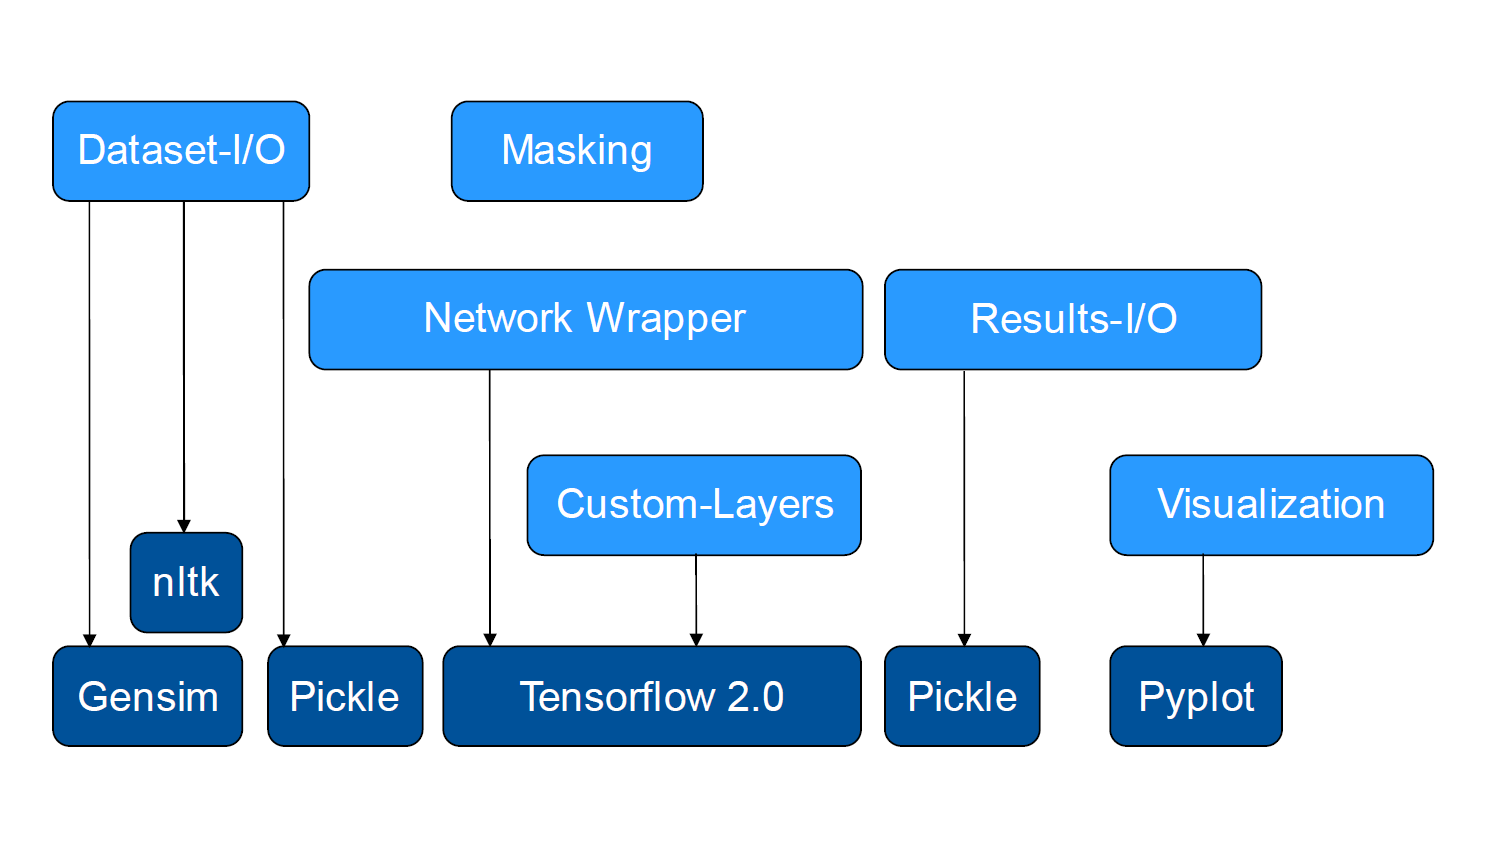
\includegraphics[width=450px]{gfx/structure2.png}
	\caption{project architecture}
	\label{fig:Interaction}
\end{figure}


\section{Summary}

%*****************************************
%**************Data Sets******************
%*****************************************
%*****************************************
\chapter{Data Sets}
\label{ch:data_sets}
%*****************************************
\begin{figure}
	\begin{tabular}{c|c|c|c|c}
		& MNIST & CIFAR-10 & 20-Newsgroup & Reuters-21578\\
		\hline
		N. labels & 10 & 10 & 20 & 10 to 115\\
		N. datapoints & 70.000 & 60.000 & 18846  & 12.902\\
		fixed split & x & x & "bydate" & "ModApt\'e"\\
		shortened &  &  & x & x\\
		class imbalance &  &  &  & x\\
		multi-label &  &  &  & x\\
	\end{tabular}
\end{figure}

\section{MNIST}
The MNIST-dataset contains 25x25 gray-scale images of handwritten digits padded to 28x28 \cite{MNIST}. 

\section{CIFAR-10}

\section{20-Newsgroup}

\section{Reuters-21578}
The Reuters-21578-dataset contains 21578 articles published by the Reuters News Agency in 1987 \cite{Reuters-21578}. Reuters-21578 differs from the previous data sets in the sense that it lacks a few fundamental properties. In particular Reuters-21578 is not only multi-class but rather multi-label meaning that any one data point can satisfy multiple categories. Additionally there are categories in Reuters-21578 that have no associated positive example and even for all remaining ones the amount of samples is heavily skewed. In order to restore parts of the missing properties with minimal change to the dataset different subsets of Reuters-21578 have been chosen by different researchers.\\
F. Debole \& F. Sebastiani \cite{Reuters-Subsets} describe those subsets, starting out stating that close to half of the data points are unusable which leaves 12,902 documents. 9,603 are marked for training and 3,299 for validation.\footnote{While different training-splits were used for Reuters-21578 "ModApt\'e" has become the canonical choice} They also point out the different groups of categories used for classification:
\begin{itemize}
	\item \textbf{R$\left(115\right)$}\\
	The group with the 115 categories containing at least one positive training example.\\ 
	\item \textbf{R$\left(90\right)$}\\
	The group with the 90 categories containing at least one positive training and test example.\\ 
	\item \textbf{R$\left(10\right)$}\\
	The group with the 10 categories containing the most examples. \\
\end{itemize} 

%*****************************************
%**************Evaluation*****************
%*****************************************
%*****************************************
\chapter{Evaluation}
\label{ch:evaluation}
%*****************************************
%\hint{This chapter should describe how the evaluation of the implemented mechanism was done. \\ \\
%1. Which evaluation method is used and why? Simulations, prototype? \\
%2. What is the goal of the evaluation? Comparison? Proof of concept? \\
%3. Wich metrics are used for characterizing the performance, costs, fairness, and efficiency of the system?\\
%4. What are the parameter settings used in the evaluation and why? If possible always justify why a certain threshold has been chose for a particular parameter.  \\
%5. What is the outcome of the evaluation? \\ \\
%The section should have a length of about five to ten pages.}
The following chapter presents the results achieved throughout this thesis and aims to explain their evaluation. First, the intended goal of each experiment is stated, including a  formulation in terms of validatable benchmarks. Subsequently, the process which extracts legible data from the framework is developed. The visualized data follows, and finally, the results are analyzed.

\section{Reproduction}
\subsection*{Goal and Benchmarks}
As the latter sections evaluate explorative experiments, the validity of the framework which supports them is crucial. We trained the first two models described in sections \ref{ch:design} and \ref{ch:implementation} under the conditions J. Frankle and M. Corbin describe in their paper. The mismatch of weights previously described forms the only known difference.
J. Frankle and M. Corbin primarily report the accuracy achieved by their implementations at the epoch of a simple stopping criterion. They executed each experiment five times and plot the mean alongside the minimum and maximum, which are represented through error bars. Additionally, they reperformed the same experiments ten times, but applied the masks, found after each epoch, to randomly reinitialized networks. The results were visualized in the same manner. \cite{LTH}
On the left side of figure 7.1 and figure 7.2, these measures are presented for the MNIST-FCN and the CIFAR10-CNN-6, respectively. Both plots are taken from the Lottery Ticket Hypothesis paper, but we cleaned up the latter one and brought it up to scale for improved legibility.\footnote{The original figure is available in the paper of J. Frankle and M. Carbin. \cite{LTH}}  The goal of this reproduction is to produce results within the reported confidence intervals of accuracy in the Lottery Ticket Hypothesis paper.  

\subsection*{Evaluation Setup}
As the produced framework does not provide any early stopping criterion, we display the full range of accuracy a given architecture achieves after convergence. A line visualizes the mean, while a gray band denotes the interval between maximal and minimal achieved accuracy. As a positive side-effect, this setup increases the breadth of visualized data in the following explorative experiments because it is parameter-agnostic concerning the early stopping criterion. Finally,  as J. Frankle and M. Corbin present training accuracies for the MNIST-Lenet-FCN architecture, we visualize the same measure for additional points of comparison.\footnote{For the Conv6 architecture, the effective pruning rate per iteration amalgamate its dense and convolutional pruning rate. The disagreement in the number of weights in the dense layers between our framework and the Lottery Ticket Hypothesis paper also results in a different pruning rate per epoch. Furthermore J. Frankle and M. Carbin arrive at slightly different pruning rate after rounding.\\ While the labels nominally differ, we visualized our data with a grid corresponding to the same amount of training or pruning. It reduces legibility but increases ease of comparison.
} 
\subsection*{Evaluation Results}
As seen in figures \ref{fig:MNIST-Lenet-FCN-LTH} and \ref{fig:MNIST-Lenet-FCN-Thesis}, the MNIST-Lenet-FCN implementation we provide achieves a lower accuracy than reported by J. Frankle and M. Corbin. Additionally, it does not show an interim improvement and degrades significantly faster at advanced pruning iterations. Said degradation is qualitatively similar to the behavior of the randomly reinitialized networks.
The comparison between figure \ref{fig:CIFAR10-Conv6-LTH} and figure \ref{fig:CIFAR10-Conv6-Thesis} yields similar results. While the CIFAR10-CNN-6 implementation produces the same accuracy as a full network, it degrades as quickly as J. Frankel and M. Corbin's reinitialized networks. Most of its graph falls into the deviation intervals they visualized.

\begin{figure}
	\begin{minipage}{\textwidth}
		\centering
		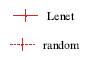
\includegraphics[width=100px]{gfx/7-Evaluation/LTH_3_legend.png}
	\end{minipage}
	\begin{minipage}{0.5\textwidth}
		\centering
		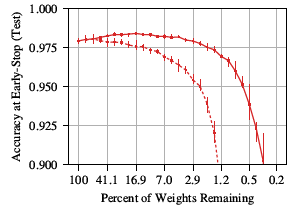
\includegraphics[height=180px]{gfx/7-Evaluation/LTH_0.png}
		\caption{LTH: MNIST-Lenet-FCN}
		\vspace{7pt}
		\footnotesize{
			Source:\\
			"The Lottery Ticket Hypothesis" \cite{LTH}
		}
		\label{fig:MNIST-Lenet-FCN-LTH}
	\end{minipage}\hfill
	\begin{minipage}{0.5\textwidth}
		\centering
		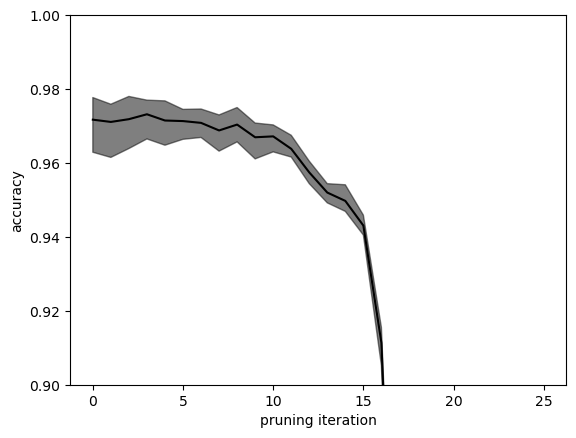
\includegraphics[height=180px]{gfx/Experiments/Reproduction-MNIST-FCN/accuracy/converged.png}
		\caption{Thes: MNIST-Lenet-FCN}
		\vspace{7pt}
		\footnotesize{
			Source:\\
			This graph was produced by the author.
		}
		\label{fig:MNIST-Lenet-FCN-Thesis}
	\end{minipage}
\end{figure}

\begin{figure}
	\begin{minipage}{\textwidth}
		\centering
		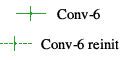
\includegraphics[width=100px]{gfx/7-Evaluation/LTH_4_legend.png}
	\end{minipage}
	\begin{minipage}{0.5\textwidth}
		\centering
		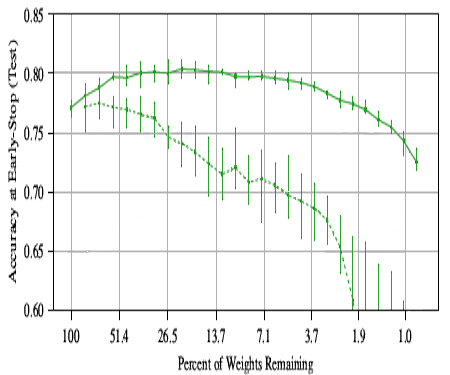
\includegraphics[height=180px]{gfx/7-Evaluation/LTH_CNN_clean.png}
		\caption{LTH: CIFAR10-Conv6}
		\vspace{7pt}
		\footnotesize{
			Source:\\
			"The Lottery Ticket Hypothesis" \cite{LTH}
		}
		\label{fig:CIFAR10-Conv6-LTH}
	\end{minipage}\hfill
	\begin{minipage}{0.5\textwidth}
		\centering
		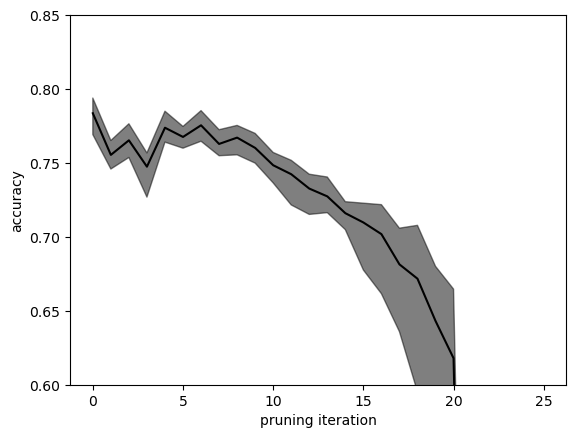
\includegraphics[height=180px]{gfx/Experiments/Reproduction-CIFAR10-CNN/accuracy/LTH.png}
		\caption{Thesis: CIFAR10-Conv6}
		\vspace{7pt}
		\footnotesize{
			Source:\\
			This graph was produced by the author.
		}
		\label{fig:CIFAR10-Conv6-Thesis}
	\end{minipage}
\end{figure}

\begin{figure}
	\begin{minipage}{\textwidth}
		\centering
		
\includegraphics[width=100px]{gfx/7-Evaluation/LTH_1_legend.png}
	\end{minipage}
	\begin{minipage}{0.5\textwidth}
		\centering
		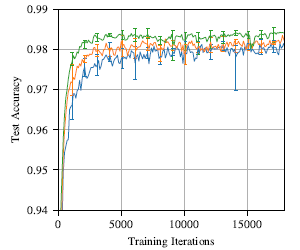
\includegraphics[height=180px]{gfx/7-Evaluation/LTH_1.png}
		\caption{LTH: Slightly pruned Lenet-FCN}
		\vspace{7pt}
		\footnotesize{
			Source:\\
			"The Lottery Ticket Hypothesis" \cite{LTH}
		}
		\label{fig:Slightly-Pruned-Lenet-LTH}
	\end{minipage}\hfill
	\begin{minipage}{0.5\textwidth}
		\centering
		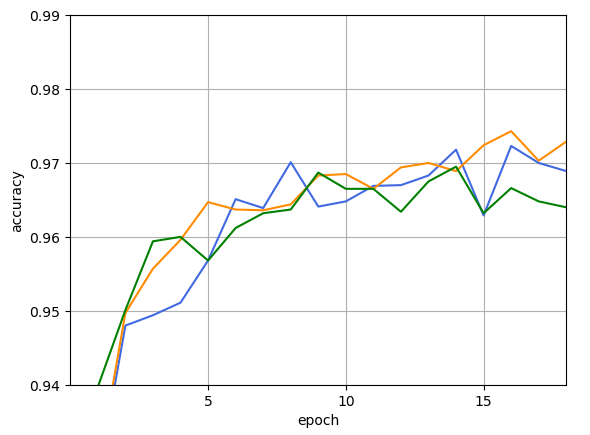
\includegraphics[height=180px]{gfx/Experiments/Reproduction-MNIST-FCN/accuracy/LTH_1.png}
		\caption{Thesis: Slightly pruned Lenet-FCN}
		\vspace{7pt}
		\footnotesize{
			Source:\\
			This graph was produced by the author. \cite{LTH}
		}
		\label{fig:Slightly-Pruned-Lenet-Thesis}
	\end{minipage}
\end{figure}

\begin{figure}
	\begin{minipage}{\textwidth}
		\centering
		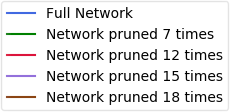
\includegraphics[width=100px]{gfx/7-Evaluation/LTH_2_legend.png}
	\end{minipage}
	\begin{minipage}{0.5\textwidth}
		\centering
		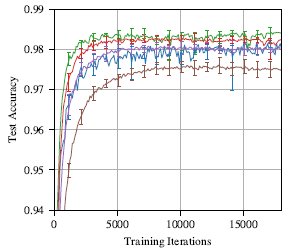
\includegraphics[height=180px]{gfx/7-Evaluation/LTH_2.png}
		\caption{LTH: Heavily pruned Lenet-FCN}
		\vspace{7pt}
		\footnotesize{
			Source:\\
			"The Lottery Ticket Hypothesis" \cite{LTH}
		}
		\label{fig:Heavily-Pruned-Lenet-LTH}
	\end{minipage}\hfill
	\begin{minipage}{0.5\textwidth}
		\centering
		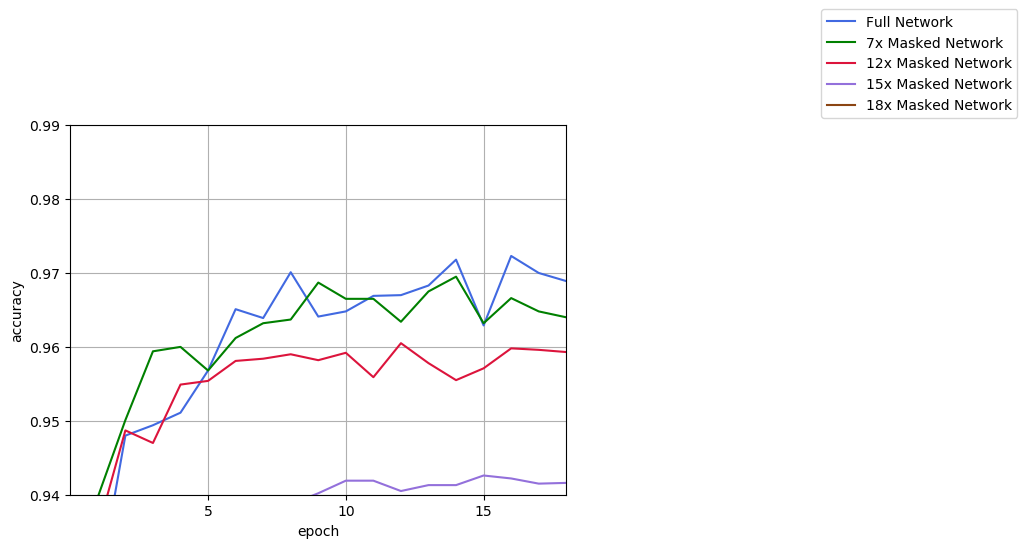
\includegraphics[height=180px]{gfx/Experiments/Reproduction-MNIST-FCN/accuracy/LTH_2.png}
		\caption{Thesis: Heavily pruned Lenet-FCN}
		\vspace{7pt}
		\footnotesize{
			Source:\\
			This graph was produced by the author.
		}
		\label{fig:Heavily-Pruned-Lenet-Thesis}
	\end{minipage}
\end{figure}

\subsection*{Analysis of Results}
The implementations of the provided framework do not reproduce the results presented in the Lottery Ticket Hypothesis paper, meaning that the framework is not validated. This poses the question of how to proceed with the remaining experiments, which we discuss in the corresponding "Goal and Benchmarks" subsections.
While the framework did not fulfill the primary goal of the experiment, two phenomena remain unclear and intriguing:
The MNIST-Lenet-FCN architecture produces through our implementation of the Lottery Ticket algorithm degrades only by one percentage point under compression of up to ten times. Such a result is comparable to various pruning methods discussed in chapter \ref{ch:relatedwork}. 

%*****************************************

\section{Transfer}
\subsection*{Goal and Benchmarks}
While the reproduction experiments did not validate the framework, it still pruned the MNIST-Lenet-FCN to a degree comparable to contemporary work through, and it did so through the masking of networks with frozen initialization. As such, the transfer to another field still might yield another pruning tool for additional tasks and applications. If the framework prunes about 90 percent of weight without the sacrifice of prediction quality, we consider the transfer succesful.
\subsection*{Evaluation Setup}
Figure \ref{fig:20Newsgroups-Converged} present benchmarks collected in the same manner as for the other architectures, but fewer pruning iterations are displayed. Additionally, figure \ref{fig:20Newsgroups-Training} provides the training accuracy we used to determine the amount of training necessary for convergence. The sheer size of the 20Newsgroups-End2End architecture severely limited the number of pruning iterations, a single experiment could afford to run without overflowing the memory of our computing devices. We managed to run experiments with ten pruning iterations, the minimal number to prune a network to a competitive degree. 
\subsection*{Evaluation Results}
The right side of figure 7.4 shows that the 20Newsgroups-End2End architecture retains its accuracy even if about 90 percent of its weights are pruned. Additionally, the networks of the intermediate pruning epochs show an accuracy improvement of at least one percentage point.
\begin{figure}
	\begin{minipage}{0.5\textwidth}
		\centering
		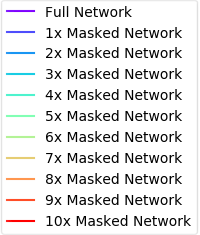
\includegraphics[width=100px]{gfx/7-Evaluation/20Newsgroups_legend.png}
	\end{minipage}
	\begin{minipage}{0.5\textwidth}
		\centering
		%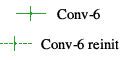
\includegraphics[width=100px]{gfx/7-Evaluation/LTH_4_legend.png}
	\end{minipage}
	\\
	\begin{minipage}{0.5\textwidth}
		\centering
		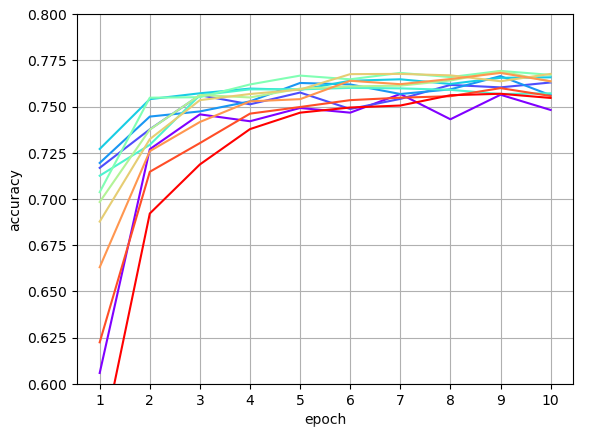
\includegraphics[height=180px]{gfx/Experiments/Transfer-20Newsgroups-CNN/accuracy/10_iterations.png}
		\caption{Training history on 20Newsgroups}
		\vspace{7pt}
		\footnotesize{
			Source:\\
			This graph was produced by the author.
		}
		\label{fig:20Newsgroups-Training}
	\end{minipage}\hfill
	\begin{minipage}{0.5\textwidth}
		\centering
		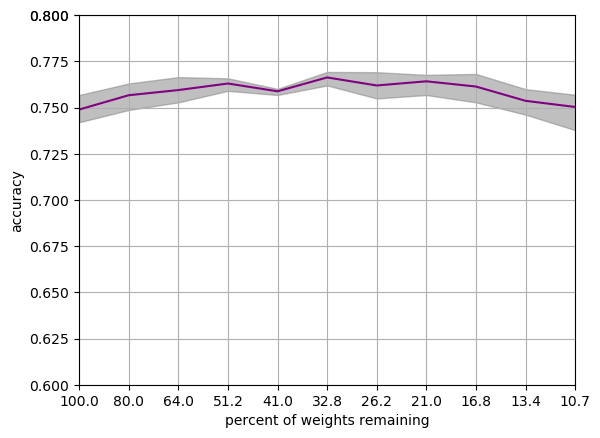
\includegraphics[height=180px]{gfx/Experiments/Transfer-20Newsgroups-CNN/accuracy/converged.png}
		\caption{Accuracy after convergence}
		\vspace{7pt}
		\footnotesize{
			Source:\\
			This graph was produced by the author.
		}
		\label{fig:20Newsgroups-Converged}
	\end{minipage}
\end{figure}

\subsection*{Analysis of Results}
According to the previously defined goal, the transfer was successful, which shows that non-image-recognition architectures can contain efficient subnetworks upon initialization.

%*****************************************
\newpage

\section{Early Tickets}
Independent of the ability to recover actual lottery tickets, the pruning implementation supplied by our framework finds small subnetworks in the initialization which are trainable to a nontrivial accuracy. H. Zhou et al. findings confirm that the utilization of trained weights, to calculate the pruning mask, is essential.\cite{Deconstructing_LTH} Information on the development of the quality of said weights is still of interest. 
\subsection*{Goal and Benchmarks}
The aim of this experiment is purely explorative. If any patterns are recognized, they may inform experiments implemented with valid frameworks.
\subsection*{Evaluation Setup}
Figures \ref{fig:Early-Tickets-0} through \ref{fig:Early-Tickets-9} plot the mean accuracy achieved by implementations set to prune at the n-th epoch of training. To avoid visual clutter, the interval representing minimal and maximal values are omitted. 
\subsection*{Evaluation Results}
Because the accuracy of multiple graphs behaves erratically, it is challenging to discern a development over the training depth. The only certain observation is that all trials of earlier pruning degrade significantly faster than the original approach.
\subsection*{Analysis of Results}
While the original network converges in about ten epochs the same amount of training does not seem to suffice to achieve the full efficiency of the pruning algorithm implemented in our framework

\newpage
\begin{figure}
	\begin{minipage}{\textwidth}
		\centering
		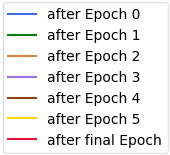
\includegraphics[width=100px]{gfx/7-Evaluation/LTH_5_legend.png}
	\end{minipage}
	\begin{minipage}{0.45\textwidth}
		\centering
		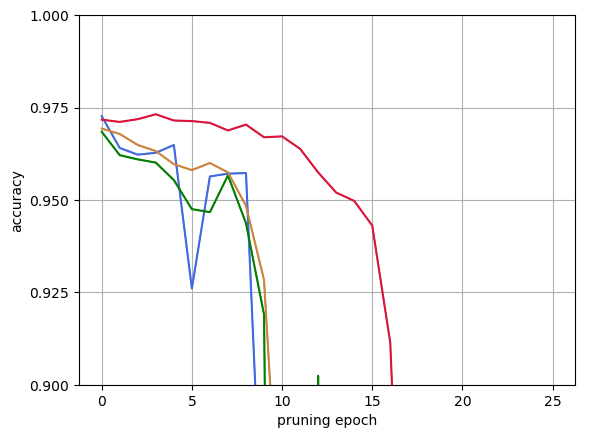
\includegraphics[height=175px]{gfx/Experiments/EarlyTicket-MNIST-FCN/012.png}
		\caption{Networks pruned at epochs 0|1|2}
		\vspace{7pt}
		\footnotesize{
			Source:\\
			This graph was produced by the author.
		}
		\label{fig:Early-Tickets-0}
	\end{minipage}\hfill
	\begin{minipage}{0.45\textwidth}
		\centering
		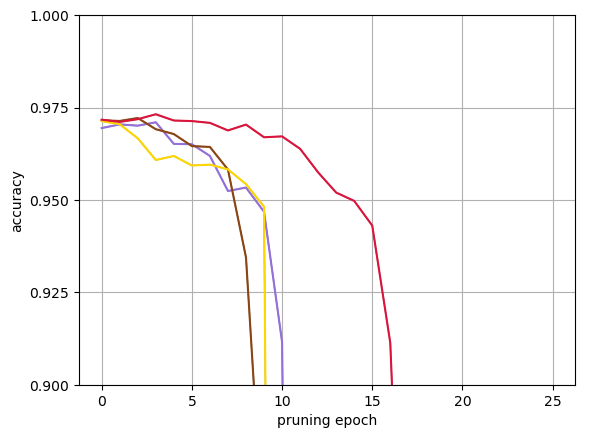
\includegraphics[height=175px]{gfx/Experiments/EarlyTicket-MNIST-FCN/345.png}
		\caption{Networks pruned at epochs 3|4|5}
		\vspace{7pt}
		\footnotesize{
			Source:\\
			This graph was produced by the author.
		}
		\label{fig:Early-Tickets-4}
	\end{minipage}
\end{figure}
\begin{figure}
	\begin{minipage}{\textwidth}
		\centering
		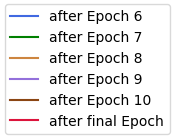
\includegraphics[width=100px]{gfx/7-Evaluation/LTH_6_legend.png}
	\end{minipage}
	\begin{minipage}{0.45\textwidth}
		\centering
		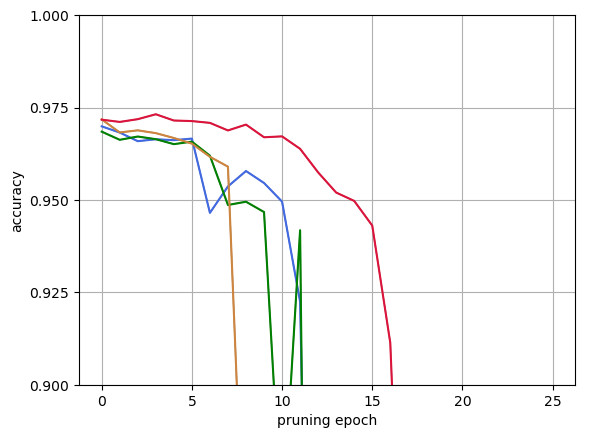
\includegraphics[height=175px]{gfx/Experiments/EarlyTicket-MNIST-FCN/678.png}
		\caption{Networks pruned at epochs 6|7|8}
		\vspace{7pt}
		\footnotesize{
			Source:\\
			This graph was produced by the author.
		}
		\label{fig:Early-Tickets-6}
	\end{minipage}\hfill
	\begin{minipage}{0.45\textwidth}
		\centering
		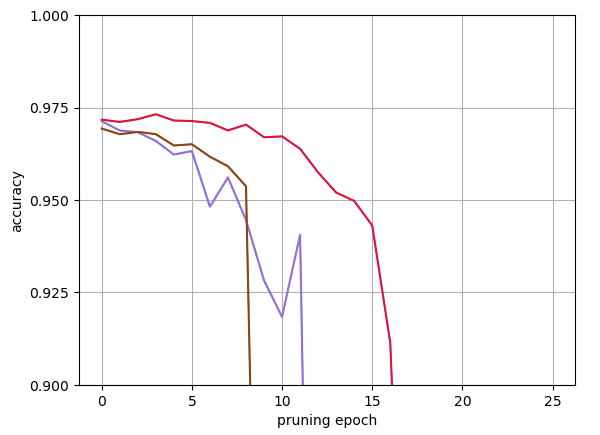
\includegraphics[height=175px]{gfx/Experiments/EarlyTicket-MNIST-FCN/910.png}
		\caption{Networks pruned at epochs 9 and 10}
		\vspace{7pt}
		\footnotesize{
			Source:\\
			This graph was produced by the author.
		}
		\label{fig:Early-Tickets-9}
	\end{minipage}
\end{figure}



%*****************************************
%**************Conclusions****************
%*****************************************
%*****************************************
\chapter{Conclusions}
\label{ch:closure}
%*****************************************

%\hint{This chapter should summarize the thesis and describe the main contributions of the thesis. Subsequently, it should %describe possible future work in the context of the thesis. What are limitations of the developed solutions? Which things can %be improved?
%The section should have a length of about three pages.}
To conclude this thesis, the following sections summarize the accomplished work, assure results and record possibilities for future work

\section{Summary}
Inspired by the paper J. Frankle and M. Corbin published at the beginning of 2019, we decided to research two applications of the pruning algorithm they proposed. With the help of Tensorflow 2.0, the natural language toolkit nltk, scikit-learn, and a few additional backend applications, we developed a framework to search different architectures for lottery tickets. Afterward, we designed four experiments: two to validate the framework, one to extend this kind of pruning to new datasets, and the last one to explore the emergence of actionable training experience in an architecture.  The reproduction was not successful, but the framework still pruned the MNIST-Lenet-FCN architecture by a factor of ten while loosing less than a percentage point. The second experiment was a definite success, and the exploration of early pruning possibilities yielded no starting points for further study.

\section{Contributions}
The primary contribution of this thesis is the openly available framework we developed. While it failed the reproduction experiments, it achieved competitive pruning results on at least two architectures. Furthermore, the availability of source code enables any future researcher to check and rerun the tests themselves. Additionally, the success of the second experiment makes a good case for the application of the presented kind of pruning algorithm in the field of natural language processing.

\section{Future Work}
The developed framework could be a convenient tool to prune various networks, but at the moment, it is heavily limited by two factors:

Firstly, some part of the workflow fills up the working memory once per pruning iteration. Experiments with massive architectures or great pruning depth may cause a memory failure resulting in the loss of all training data. Our best guess for a cause is the Tensorflow 2.0 backend. During the restoration of weight after one training procedure has finished, it might integrate the newly pruned model into its old execution graph instead of creating a new one.

Secondly, the lack of a fourth layer of abstraction overloads the main module. As described in chapter [5], the framework function at three such layers, but none of them should handle the control flow between and visualization. The result is an inefficient way to interface with the framework.

Finally, the success of the transfer experiment shows that the implemented pruning methodology can extend to non-image datasets. The next sensible point of order is a proof-of-concept that the method can also be extended to architectures more common in the natural language processing field, such as LSTMs.

%\section{Final Remarks}
